\begin{figure}[H]
\centering
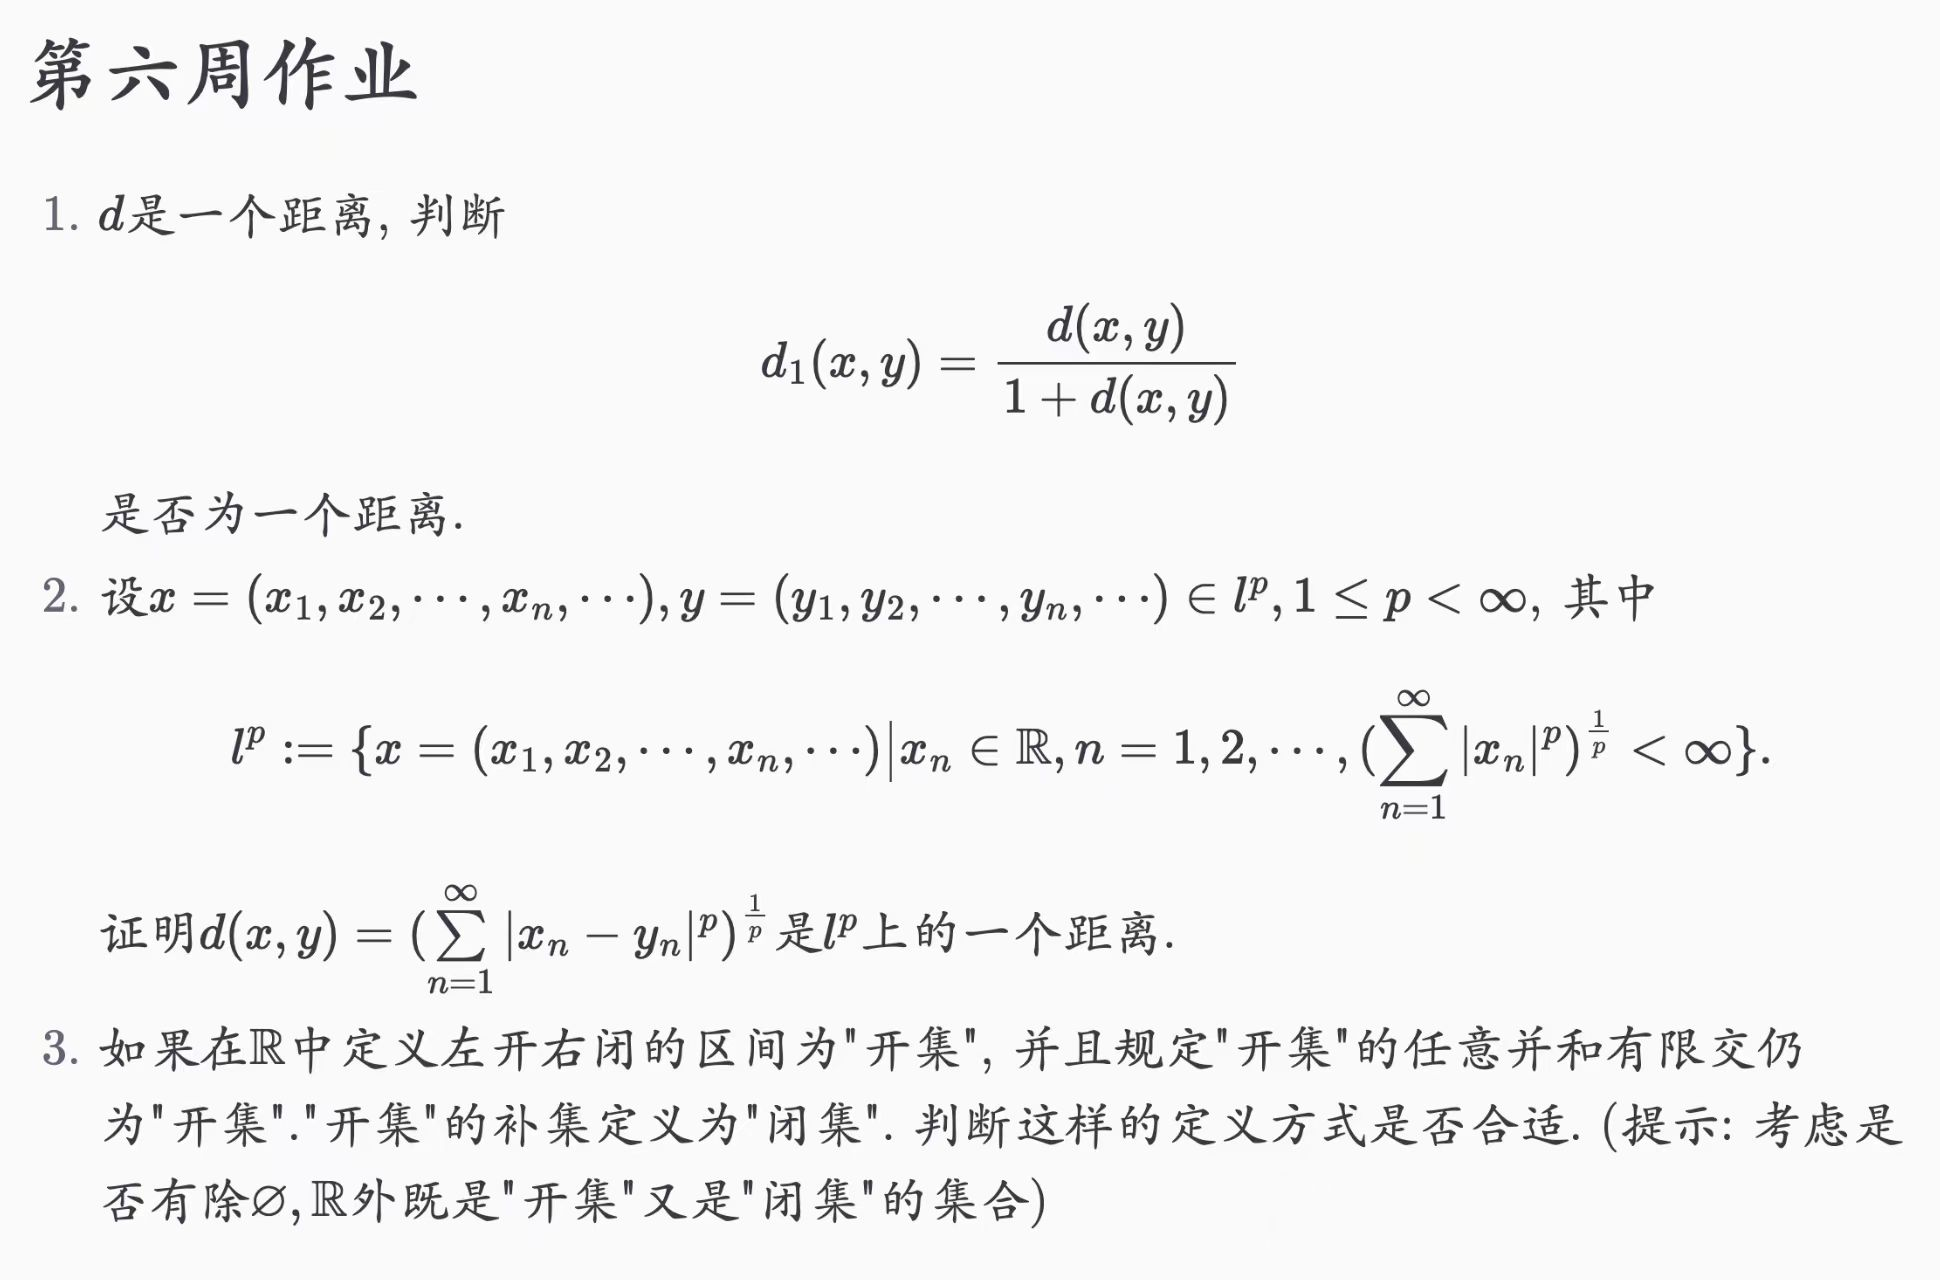
\includegraphics[width=\textwidth]{d64b9372e28853ce2a9c54e98cf4a55.jpg}
% \caption{}
\label{}
\end{figure}

\begin{exercise}
\begin{figure}[H]
\centering

\includegraphics[width=\textwidth]{hw6-2025040420.png}
% \caption{}
\label{}
\end{figure}
\end{exercise}
\begin{figure}[H]
\centering
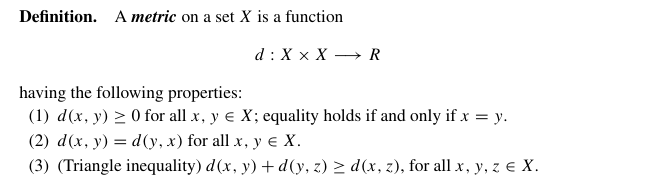
\includegraphics[width=\textwidth]{2-hw6-2025040420.png}
% \caption{}
\label{}
\end{figure}

(1) 显然 $d_1(x,y)\geq0$ 且
\[
d_1(x,y)=0\iff d(x,y)=0\iff x=y
\]
(2) 显然 $d_1(x,y)=d_1(y,x)$

(3) 不妨设 $d(x,y)\geq d(y,z)$,若 $d(x,y)\geq d(x,z)$ 那么显然有
\[
\frac{d(x,y)}{1+d(x,y)}+\frac{d(y,z)}{1+d(y,z)}\geq \frac{d(x,z)}{1+d(x,z)}
\]
若 $d(x,y)<d(x,z)$,则
\[
\frac{d(x,y)}{1+d(x,y)}+\frac{d(y,z)}{1+d(y,z)}\geq \frac{d(x,y)}{1+d(x,z)}+\frac{d(y,z)}{1+d(x,z)}\geq \frac{d(x,z)}{1+d(x,z)}
\]
因此 $d_1$ 是一个距离.

\begin{exercise}
\begin{figure}[H]
\centering
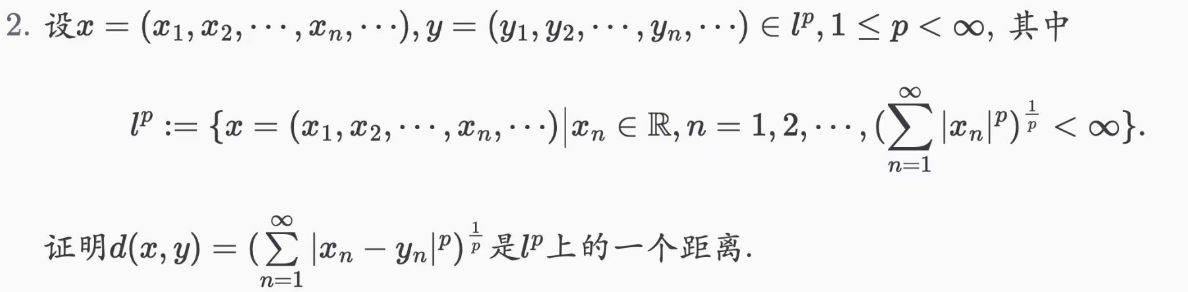
\includegraphics[width=\textwidth]{3-hw6-2025040420.png}
% \caption{}
\label{}
\end{figure}
\end{exercise}
\begin{figure}[H]
\centering
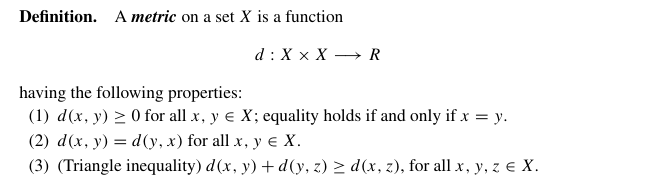
\includegraphics[width=\textwidth]{2-hw6-2025040420.png}
% \caption{}
\label{}
\end{figure}
(1) 显然 $d(x,y)\geq0$,若 $d(x,y)=\left( \sum_{n=1}^{\infty}\lvert x_n-y_n \rvert ^{p} \right)^{1/p}=0$,那么 $x_n=y_n,\forall n$. 因此 $x=y$.

(2) 显然 $d(x,y)=d(y,x)$.

(3)
\[
\begin{aligned}
d(x,y)+d(y,z) & =\left( \sum_{n=1}^{\infty} \lvert x_n-y_n \rvert ^{p} \right)^{1/p }+\left( \sum_{n=1}^{\infty} \lvert y_n-z_n \rvert ^{p} \right)^{1/p } \\
 & \geq \left( \sum_{n=1}^{\infty} (\lvert x_n-y_n \rvert +\lvert y_n-z_n \rvert )^{p} \right)^{1/p } \\
 & \geq \left( \sum_{n=1}^{\infty} \lvert x_n-z_n \rvert ^{p}  \right)^{1/p }=d(x,z) 
\end{aligned}
\]
因此 $d(x,y)$ 是 $l^{p}$ 上的一个距离.

\begin{exercise}
\begin{figure}[H]
\centering

\includegraphics[width=\textwidth]{4-hw6-2025040420.png}
% \caption{}
\label{}
\end{figure}
\end{exercise}
$(0,1]$ 是开集,则 $(-\infty,0]\cup(1,+\infty)$ 是闭集,但是
\[
(-\infty,0]\cup(1,+\infty)=\bigcup_{n=2}^{\infty}\underbrace{ ((-n,0] \cup(1,n]) }_{ \text{open} }
\]
故 $(-\infty,0]\cup(1,+\infty)$ 是开集,故 $(0,1]$ 既开又闭,但不是全集也不是空集. 这样的定义不合适
